\documentclass[xcolor=table]{beamer}
\beamertemplatenavigationsymbolsempty
\setbeamertemplate{blocks}[rounded=true, shadow=true]
\setbeamertemplate{footline}[page number]
\usecolortheme{beaver}

\usepackage{fontspec}
% enable the traditional TeX ligatures:
\defaultfontfeatures{Ligatures=TeX}
\setmainfont{Times New Roman}
\setsansfont{Arial}
\setmonofont[Script=Cyrillic]{DejaVu Sans Mono}

\newfontfamily\cyrillicfont{Times New Roman}
\newfontfamily\cyrillicfontsf{Times New Roman}

\usepackage{unicode-math}
\setmathfont{TeX Gyre Termes Math} 

\usepackage{polyglossia}
\setmainlanguage{russian}
\setotherlanguage{english}

\usepackage[backend=biber, style=authoryear, url=false, isbn=false]{biblatex}
\addbibresource{references.bib}

\usepackage{amssymb,amsfonts,amsmath}
\usepackage{algorithmic}
\usepackage{subfig}
\usepackage[all]{xy}
\usepackage{array}
\usepackage{tikz}
\usepackage{multicol}
\usepackage{hyperref}
\usepackage{hhline}
\usepackage{booktabs}  % красивые линии
\usepackage{makecell}  % многострочные ячейки

\graphicspath{{fig/}{../fig/}}

\DeclareMathOperator*{\argmax}{arg\,max}
\DeclareMathOperator*{\argmin}{arg\,min}


% A handy helper to put four graphics in a 2×2 grid (no extra packages needed).
% Usage: \quadgraphics{file1}{file2}{file3}{file4}
\newcommand{\quadgraphics}[4]{%
  \begin{columns}[T,onlytextwidth]
    \column{0.48\textwidth}
      \includegraphics[width=\linewidth]{#1}\\[0.5em]
      \includegraphics[width=\linewidth]{#3}
    \column{0.48\textwidth}
      \includegraphics[width=\linewidth]{#2}\\[0.5em]
      \includegraphics[width=\linewidth]{#4}
  \end{columns}}

%----------------------------------------------------------------------------------------------------------
\title{Untangling Equifinality: A Large-Sample Benchmark of Machine-Learning Models for Rainfall–Runoff Forecasting in Eurasian Basins}
\author[Э.~Хузин]{Эльдар Хузин}
\institute{Московский физико-технический институт}
\date{\footnotesize
\par\smallskip\emph{Курс:} My first scientific paper
\par\smallskip\emph{Эксперт:} Д.~Абрамов
\par\smallskip\emph{Консультант:} Д.~Абрамов
\par\bigskip\small 2025}

\begin{document}

\begin{frame}[plain]
    \maketitle
\end{frame}
%-----------------------------------------------------------------------------------------------------
\begin{frame}{Цель исследования}
    \begin{block}{Цель}
        Исследовать эквифинальность моделей RF, XGBoost, LSTM, а также их способность выявлять гидрологические закономерности.
    \end{block}

    \begin{block}{Задача}
        Сравнить одинаковые по точности модели в их способности выделять ключевые для бассейнов статические характеристики.
    \end{block}

    \begin{block}{Решение}
        \begin{enumerate}
            \item На обширном датасете кластеризовать бассейны рек по статически признакам.
            \item Сравнить модели по метрикам NSE, RMSE, MAE, MAPE.
            \item Оценить вклад признаков через SHAP-значения.
            \item Проанализировать компромисс ``точность\textbackslash вычислительная
                  сложность\textbackslash интерпретируемость''.
        \end{enumerate}
    \end{block}
\end{frame}

%----------------------------------------------------------------------------------------------------------
\begin{frame}{Публикации по теме}
    \nocite{
        bevenFutureDistributedModels1992a,
        kratzertLearningUniversalRegional2019,
        SpatialtemporalBehaviorPrecipitation2022,
        % underwoodMachineLearningRevealsEquifinality2023,
        % janssenTacklingWaterTable2024,
    }
    \printbibliography[heading=None]
\end{frame}

%----------------------------------------------------------------------------------------------------------
\begin{frame}{Вычислительный эксперимент}
    \begin{enumerate}
        \item Предобработка данных
              \begin{enumerate}
                  \item Корреляционный анализ и отбор статических признаков
                  \item Заполнение пропусков
                  \item Добавление лагов и статических атрибутов
              \end{enumerate}
        \item Обучение
              \begin{enumerate}
                  \item Выделение выборок (12/3)
                  \item Подбор гиперпараметров (Optuna)
                  \item Training
              \end{enumerate}
        \item SHAP-анализ и другие метрики    \[
                  \phi_i=\!\!\!\sum_{S\subseteq N\setminus\{i\}}
                  \frac{|S|!\,(|N|-|S|-1)!}{|N|!}\;
                  \bigl[f(S\cup\{i\})-f(S)\bigr]
              \]
    \end{enumerate}
\end{frame}


%----------------------------------------------------------------------------------------------------------
\begin{frame}{Данные}
    % --- карта --------------------------------------------------
    
\includegraphics[width=\linewidth]{bin/train_gauges_cartopy_10m_clusters.pdf}

    \vspace{0.6em} % небольшой отступ

    % --- таблица (две строки) -----------------------------------
    \scriptsize
    \setlength{\extrarowheight}{2pt}
    \begin{tabular}{ccc}
        \toprule
        \textbf{Cluster} & \textbf{Rank 1}               & \textbf{Rank 2}              \\
        \midrule
        0                & lat (Широта)                  & for\_pc\_sse (Площадь лесов) \\
        1                & crp\_pc\_sse (Пахотные земли) & pst\_pc\_sse (Пастбища)      \\
        2                & gwt\_cm\_sav (Глубина ГВ)     & for\_pc\_sse (Площадь лесов) \\[2pt]
        \bottomrule
    \end{tabular}
\end{frame}
%------------------------------------------------------

%----------------------------------------------------------------------------------------------------------
\begin{frame}{Данные}
    Ежедневные данные за период с 2008 по 2022 год с 1072 бассейнов.

    \medskip
    \textbf{prcp} – количество осадков (мм/сут)\\
    \textbf{lvl\_sm} – уровень воды в реке (м) [deprecated]\\
    \textbf{t\_min} – минимальная температура (°C)\\
    \textbf{t\_max} – максимальная температура (°C)\\
    \textbf{t\_mean} – средняя температура (от почасовой) (°C)\\
    \textbf{q\_mm\_day} – расход воды (мм/сут)\\
\end{frame}

\begin{frame}{Данные}
    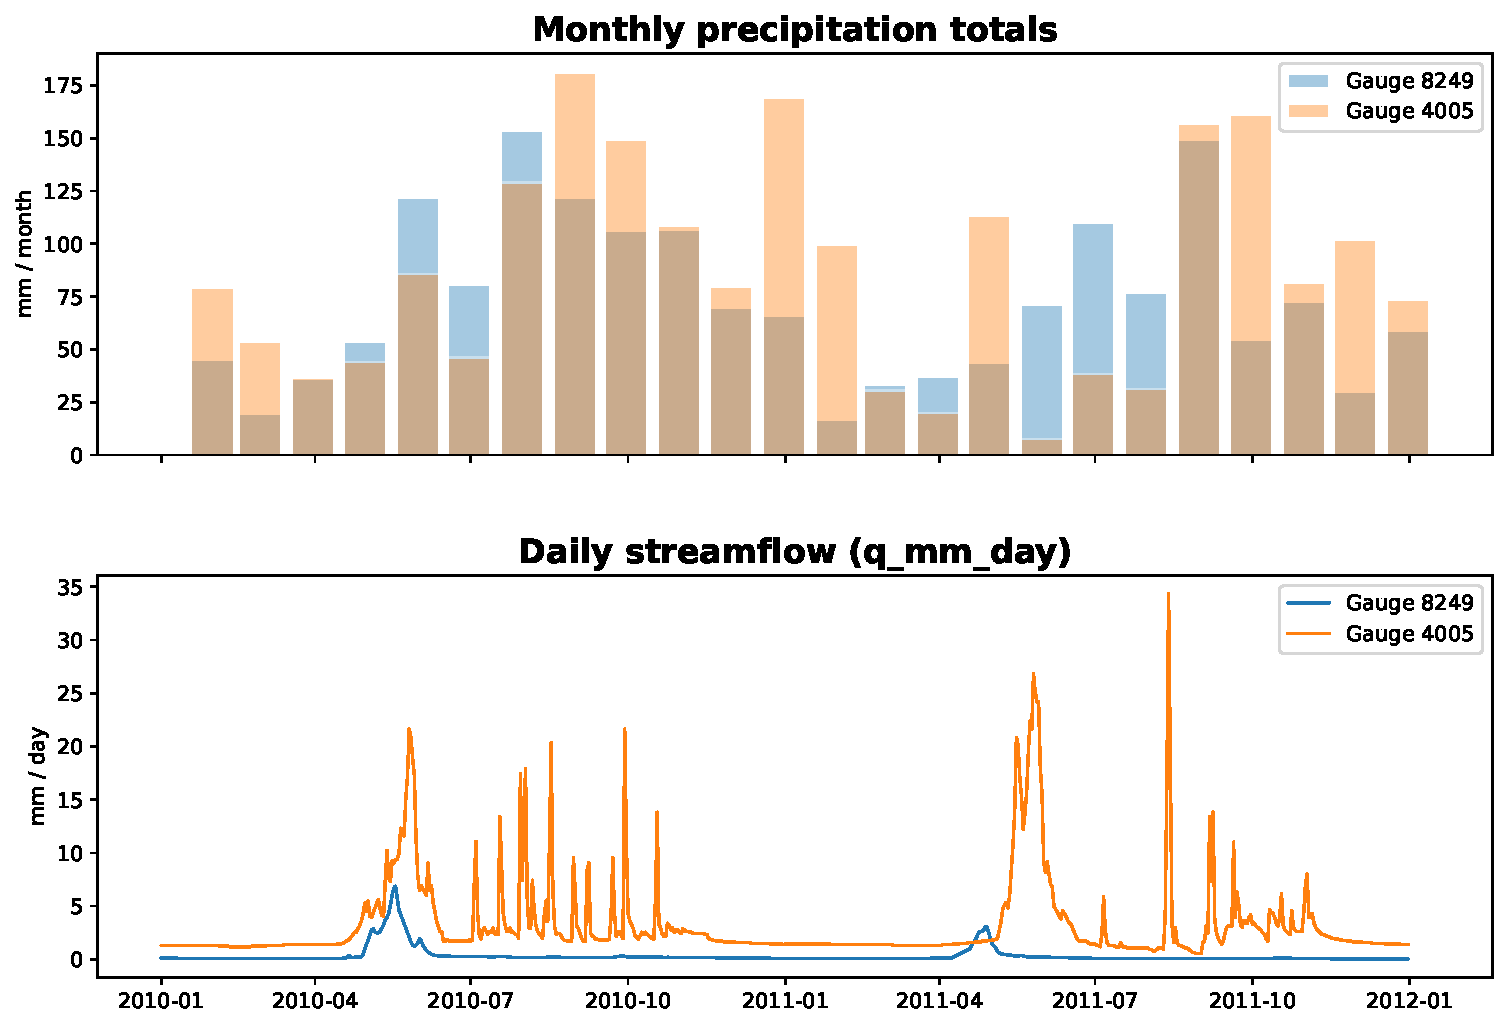
\includegraphics[width=1\textwidth]{bin/target_time_series.pdf}
\end{frame}

%----------------------------------------------------------------------------------------------------------
\begin{frame}{Описание атрибутов}
    \begin{table}[ht]
        \centering
        \begin{tabular}{lll}
            \toprule
            \textbf{ID} & \textbf{Атрибут}                     &              \\
            \midrule
            S03         & Песок в почве (\%)                   & snd\_pc\_sav \\
            S01         & Глина в почве (\%)                   & cly\_pc\_sav \\
            S02         & Ил в почве (\%)                      & slt\_pc\_sav \\
            H05         & Объём озёр (млн м$^{3}$)             & lkv\_mc\_usu \\
            H06         & Объём водохранилищ (млн м$^{3}$)     & rev\_mc\_usu \\
            H04         & Доля озёрной поверхности (\%)        & lka\_pc\_use \\
            H03         & Площадь затопления (\%)              & inu\_pc\_ult \\
            H10         & Глубина грунтовых вод (см)           & gwt\_cm\_sav \\
            H08         & Площадь рек (га)                     & ws\_area     \\
            P04         & Географическая широта ($^{\circ}$)   & lat          \\
            P05         & Географическая долгота ($^{\circ}$)  & lon          \\
            P01         & Средняя высота над уровнем моря (м)  & ele\_mt\_sav \\
            P02         & Средний уклон местности ($^{\circ}$) & slp\_dg\_sav \\
            % P03         & Средний уклон руслового профиля ($^{\circ}$) & sgr\_dk\_sav \\
            % –           & Средняя высота водосборного бассейна (м)     & height\_bs   \\
            % L07         & Лесные территории (\%)                       & for\_pc\_sse \\
            % L08         & Сельскохозяйственные угодья (\%)             & crp\_pc\_sse \\
            % L09         & Пастбища (\%)                                & pst\_pc\_sse \\
            % L10         & Орошаемые земли (\%)                         & ire\_pc\_sse \\
            % L12         & Территории вечной мерзлоты (\%)              & prm\_pc\_sse \\
            % A03         & Урбанизированные территории (\%)             & urb\_pc\_sse \\
            % S07         & Карстовые ландшафты (\%)                     & kar\_pc\_sse \\
            \bottomrule
        \end{tabular}
    \end{table}
\end{frame}


%----------------------------------------------------------------------------------------------------------
\begin{frame}{Данные}
    
\includegraphics[height=0.7\textwidth]{bin/static_selected_features_heatmap.pdf}
\end{frame}

%----------------------------------------------------------------------------------------------------------
\begin{frame}{Формальная постановка задачи}
    \begin{itemize}
        \item Предсказать $y$ на основе признаков $x$.
        \item Пусть $y \in \mathbb{R}^n$; $x \in \mathbb{R}^{n\times d}$;
        \item Набор данных: $\mathcal{D} = \{(x_i,y_i) \mid i=1,\dots,n\}$;
        \item Класс моделей: $\mathcal{F}$;
        \item Оценка: $\hat y_i = f(x_i),\; f\in\mathcal{F}$, $\hat y = (f(x_1),\dots,f(x_n))$.
    \end{itemize}
    \begin{align}
        f^* & = \argmin_{f\in\mathcal{F}} \left( \mathcal{L}(f,\mathcal{D}) + \Omega(f) \right)
    \end{align}
\end{frame}

%----------------------------------------------------------------------------------------------------------
\begin{frame}{Random Forest и Gradient Boosting}
    Модель:
    \[
        f(x) = \sum_{l=1}^L \omega_l \,\mathbb{I}(x\in R_l).
    \]
    Построение разбиений по критерию:
    \[
        \mathcal{IG}(t,j)
        = \frac12 \Bigl[ \frac{(G_L)^2}{H_L+\lambda}
            + \frac{(G_R)^2}{H_R+\lambda}
            - \frac{G^2}{H+\lambda} \Bigr] - \gamma,
    \]
    где $G_{L,R},H_{L,R}$ — суммы градиентов и гессианов.

    \begin{columns}[t,onlytextwidth]
        % ---------- Случайный лес ----------
        \column{0.48\textwidth}
        \begin{block}{Random Forest}
            \[
                f_{\mathrm{RF}}(x)=\frac{1}{B}\sum_{b=1}^{B} f^{(b)}(x)
            \]

        \end{block}

        % ---------- Градиентный бустинг ----------
        \column{0.48\textwidth}
        \begin{block}{Gradient Boosting}
            \[
                f_{\mathrm{GB}}(x)=f^{(0)}(x)+\nu\sum_{b=1}^{B} f^{(b)}(x)
            \]

        \end{block}
    \end{columns}
\end{frame}

%----------------------------------------------------------------------------------------------------------
\begin{frame}{Лосс и метрики}
    \small

    % --- MAPE ----------------------------------------------------------
    \[
        \textbf{MAPE}\;=\;\frac{1}{n}\sum_{i=1}^{n}\left|\frac{\hat{y}_{i}-y_{i}}{y_{i}}\right|
    \]

    % --- Pseudo-MAPE ---------------------------------------------------
    \[
        \textbf{Pseudo-MAPE}_{\delta}\;=\;\frac{1}{n}\sum_{i=1}^{n}\left(\sqrt{\left(\tfrac{\hat{y}_{i}-y_{i}}{y_{i}}\right)^{2}+\delta^{2}}-\delta\right)
    \]

    % --- Nash–Sutcliffe Efficiency ------------------------------------
    \[
        \textbf{NSE}\;=\;1-\frac{\sum_{i=1}^{n}(y_{i}-\hat{y}_{i})^{2}}{\sum_{i=1}^{n}(y_{i}-\bar{y})^{2}},\quad\bar{y}=\frac{1}{n}\sum_{i=1}^{n}y_{i}
    \]
\end{frame}


%----------------------------------------------------------------------------------------------------------
\begin{frame}{MAPE и Pseudo-MAPE}
    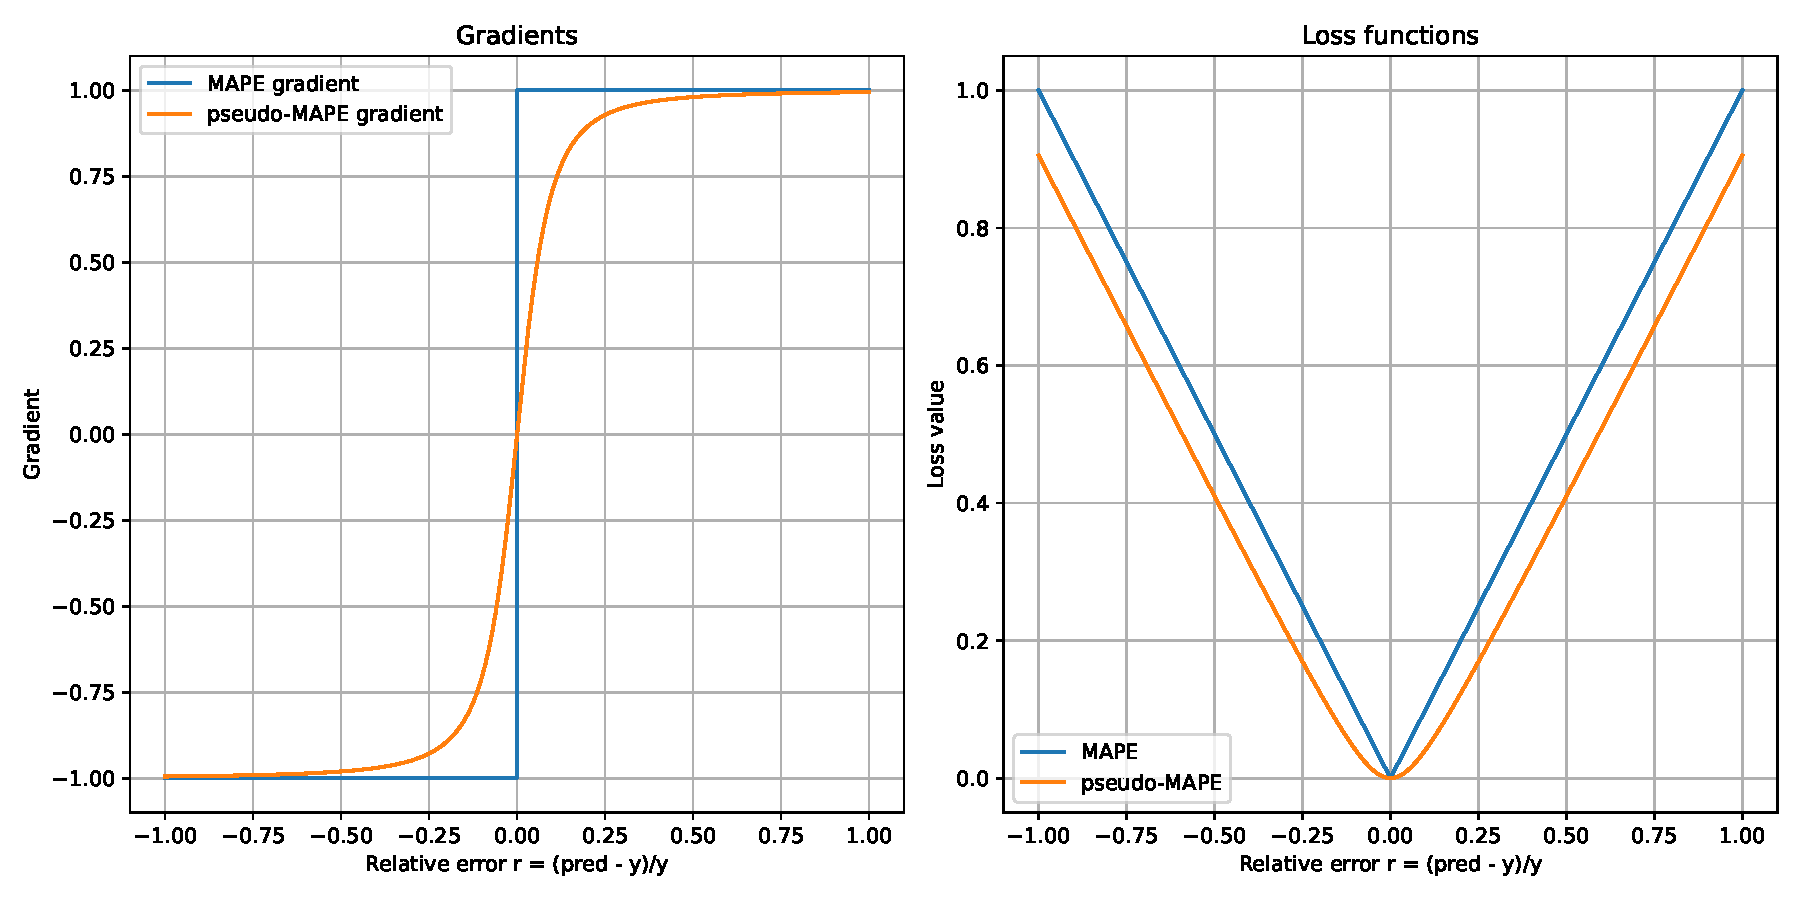
\includegraphics[width=1\textwidth]{bin/mape_vs_pseudo_mape.pdf}
\end{frame}

%----------------------------------------------------------------------------------------------------------
% ============================================================
% Boosting frames (example – extend as needed)
% ============================================================

% \begin{frame}{Результаты: Random Forest}
%     \quadgraphics{bin/shap_plots/forest/shap\_top100.pdf}%
%     {bin/shap_plots/forest/shap\_top101.pdf}%
%     {bin/shap_plots/forest/shap\_top102.pdf}%
%     {bin/shap_plots/forest/shap\_top103.pdf}
% \end{frame}
%-------------------------------------------------
% Gradient Boosting – per-cluster results
%-------------------------------------------------
% One slide: Boosting (top) + Forest (bottom)

\begin{frame}{Результаты}
    \centering
    
\includegraphics[width=\textwidth]{/home/khuzin/Projects/2025-Project-188/slides/bin/forest_prediction.pdf}
    \vspace{0.3cm}      % adjust spacing as you like
    
\includegraphics[width=\textwidth]{/home/khuzin/Projects/2025-Project-188/slides/bin/Gradient_prediction.pdf}\par
\end{frame}

\begin{frame}{Результаты}
    \centering

    %----------- Gradient Boosting ---------------
    \textbf{Gradient Boosting}\\[0.2cm]
    \begin{tabular}{
            l    % cluster
            c    % NSE
            c    % RMSE
            c    % MAE
            c    % MAPE
            r    % n_samples
        }
        \toprule
        \textbf{cluster} & \textbf{NSE} & \textbf{RMSE} & \textbf{MAE} & \textbf{MAPE} & \textbf{\#} \\
        \midrule
        0                & 0.780        & 0.577         & 0.259        & 0.655         & 44\,544     \\
        1                & 0.634        & 0.372         & 0.143        & 1.228         & 38\,371     \\
        2                & 0.820        & 0.214         & 0.120        & 0.454         & 1\,096      \\
        3                & 0.829        & 0.708         & 0.325        & 1.093         & 12\,583     \\
        \bottomrule
    \end{tabular}

    \vspace{1.0em}  % small vertical gap

    %----------- Random Forest -------------------
    \textbf{Random Forest}\\[0.2cm]
    \begin{tabular}{
            l
            c
            c
            c
            c
            r
        }
        \toprule
        \textbf{cluster} & \textbf{NSE} & \textbf{RMSE} & \textbf{MAE} & \textbf{MAPE} & \textbf{\#} \\
        \midrule
        0                & 0.922        & 0.343         & 0.149        & 0.428         & 44\,544     \\
        1                & 0.909        & 0.185         & 0.070        & 0.590         & 38\,371     \\
        2                & 0.950        & 0.112         & 0.052        & 0.173         & 1\,096      \\
        3                & 0.939        & 0.424         & 0.158        & 0.653         & 12\,583     \\
        \bottomrule
    \end{tabular}
\end{frame}

% --- first four bar plots (bar0–bar3) ----------------------------------------
\begin{frame}{Результаты: Gradient Boosting}
    \quadgraphics{/home/khuzin/Projects/2025-Project-188/slides/bin/shaps/gb/shap_top10_0.pdf}%
    {/home/khuzin/Projects/2025-Project-188/slides/bin/shaps/gb/shap_top10_1.pdf}%
    {/home/khuzin/Projects/2025-Project-188/slides/bin/shaps/gb/shap_top10_2.pdf}%
    {/home/khuzin/Projects/2025-Project-188/slides/bin/shaps/gb/shap_top10_3.pdf}%
\end{frame}

% % --- next two bar plots + overall summaries ----------------------------------
% \begin{frame}{Результаты: Gradient Boosting}
%     \quadgraphics
%     {bin/shap_plots/boosting/shap\_top102.pdf}%
%     {bin/shap_plots/boosting/shap\_top103.pdf}
% \end{frame}

% ============================================================
% Random‑Forest frames (mirror of above)
% ============================================================
\begin{frame}{Результаты: Random Forest}
    \quadgraphics{/home/khuzin/Projects/2025-Project-188/slides/bin/shaps/rf/shap_top10_0.pdf}%
    {/home/khuzin/Projects/2025-Project-188/slides/bin/shaps/rf/shap_top10_1.pdf}%
    {/home/khuzin/Projects/2025-Project-188/slides/bin/shaps/rf/shap_top10_2.pdf}%
    {/home/khuzin/Projects/2025-Project-188/slides/bin/shaps/rf/shap_top10_3.pdf}%
\end{frame}


%------------------------------------------------------------------------------------
\begin{frame}{Заключение}
    \begin{itemize}
        \item Выделенные моделями признаки не совпадают с основными кластеров, что требует дальнейшего изучения.
        \item Проявление эквифинальности наблюдалось в ходе проведения экспериментов, особенно с использованием Random Forest.
    \end{itemize}
\end{frame}
%----------------------------------------------------------------------------------------------------------
\end{document}